\section{DESIGN DE INTERFACE E TELAS DO SISTEMA WeFIND}

O design de interface de uma aplicação de utilidade pública desempenha papel determinante em sua eficácia, especialmente em situações de estresse e emergência provocadas pelo sumiço de um animal doméstico. Como ensinam Rogers, Sharp e Preece (2023), o projeto de interação deve criar experiências de uso fluidas, intuitivas e acolhedoras, minimizando a carga cognitiva exigida do usuário.

No desenvolvimento do WeFIND, o projeto gráfico e visual foi orientado pelas diretrizes de usabilidade da norma ABNT NBR ISO 9241-11 (ABNT, 2021) e pelos padrões de contraste e acessibilidade das diretrizes internacionais WCAG (W3C, 2023). A concepção priorizou a clareza nas informações, botões amplos adequados para o toque na tela de smartphones e elevado contraste para assegurar a legibilidade sob luz solar direta em ambientes abertos.

\subsection{Tipografia e Hierarquia Visual}

A escolha da tipografia estabeleceu a primeira base do design de interface do WeFIND, visto que a clareza na leitura rápida dos textos de alerta e dados de identificação dos animais é prioritária em um aplicativo de busca. A Figura~\ref{fig:tipografia} apresenta a família tipográfica adotada na aplicação.

\begin{figure}[H]
    \centering
    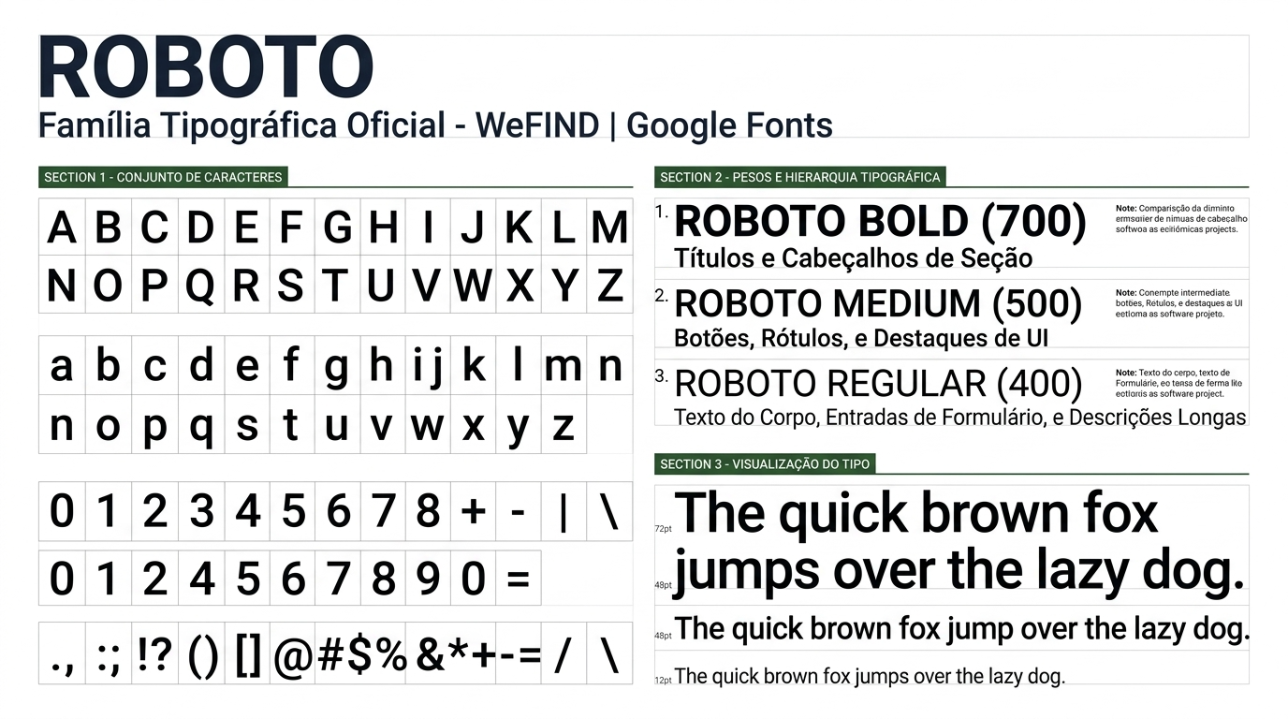
\includegraphics[width=0.99\textwidth]{imagens/03_arquitetura_design/figura15_tipografia_roboto.png}
    \caption{Família Tipográfica Roboto Adotada no WeFIND}
    \label{fig:tipografia}
    \fonte{Google Fonts (2024)}
\end{figure}

Adotou-se a família tipográfica sem serifa Roboto (GOOGLE FONTS, 2024), consagrada no design para sistemas móveis por suas proporções geométricas equilibradas e excelente legibilidade em telas de diferentes dimensões e resoluções. A organização da interface fundamenta-se em uma hierarquia visual intuitiva: os títulos e termos de destaque utilizam o peso em negrito (Bold), os botões de ação e indicadores de status empregam o peso médio (Medium), e os corpos de texto descritivos, campos de formulário e orientações operacionais utilizam o peso normal (Regular), mantendo espaçamento entre linhas suficiente para uma leitura confortável.

\subsection{Identidade Visual e Conceito do Aplicativo}

A identidade visual do WeFIND foi projetada para transmitir sentimentos de solidariedade, segurança e esperança. A própria denominação da plataforma une o pronome coletivo em língua inglesa ``We'' (Nós) ao verbo ``Find'' (Encontrar), expressando a premissa de que o resgate de um animal de estimação constitui um esforço compartilhado entre toda a comunidade.

Para a concepção do ícone e símbolo gráfico oficial, utilizou-se a ferramenta de inteligência artificial generativa Flow Labs (FLOW LABS, 2026), explorada por meio de engenharia de prompt iterativa no Figma. Os critérios solicitados ao modelo incluíram estilo visual minimalista e plano apropriado para ícones móveis, integração harmoniosa das duas espécies assistidas pela plataforma por meio das silhuetas de um cão e de um gato, presença centralizada do marcador clássico de mapa como representação da busca espacial ativa por GPS, e predomínio das cores institucionais verde floresta e terracota sobre fundo branco puro.

O prompt textual que convergiu de maneira satisfatória para esses requisitos visuais foi estruturado nos seguintes termos:

\begin{quote}
\small\textit{``Minimalist flat app icon for a lost and found pet mobile app, combining a friendly dog silhouette and a cat silhouette surrounding a central GPS location pin, solid colors forest green and terracotta, clean white background, modern vector logo design, no gradients, no photorealism.''}
\end{quote}

A partir do vetor gerado, realizou-se o refinamento geométrico e alinhamento no software Figma, estabelecendo a representação visual oficial apresentada na Figura~\ref{fig:logotipo}.

\begin{figure}[H]
    \centering
    
\includegraphics[width=0.65\textwidth]{imagens/03_arquitetura_design/figura13_logotipo_wefind.png}
    \caption{Logotipo Oficial e Ícone do Aplicativo WeFIND}
    \label{fig:logotipo}
    \fonte{Autoria própria (2026)}
\end{figure}

O símbolo gráfico reúne a silhueta de um cão à esquerda e de um gato à direita, circundando o marcador clássico de localização geográfica ao centro. Essa composição sintetiza a missão do sistema de atender às principais espécies domésticas, enquanto o marcador central enfatiza o recurso de geolocalização em mapa. As cores aplicadas reforçam a proposta: o tom Terracota acolhe as silhuetas dos animais e o Verde Esperança colore o pino de localização.

\subsection{Paleta Cromática Oficial}

A definição cromática do WeFIND baseou-se nos princípios da psicologia das cores aplicados ao design digital (HELLER, 2021), buscando transmitir serenidade e afeto sem prejudicar a visibilidade de avisos urgentes. A Figura~\ref{fig:paleta_cores} apresenta a paleta oficial, organizada em cores institucionais, cores funcionais e cores de interface.

\begin{figure}[H]
    \centering
    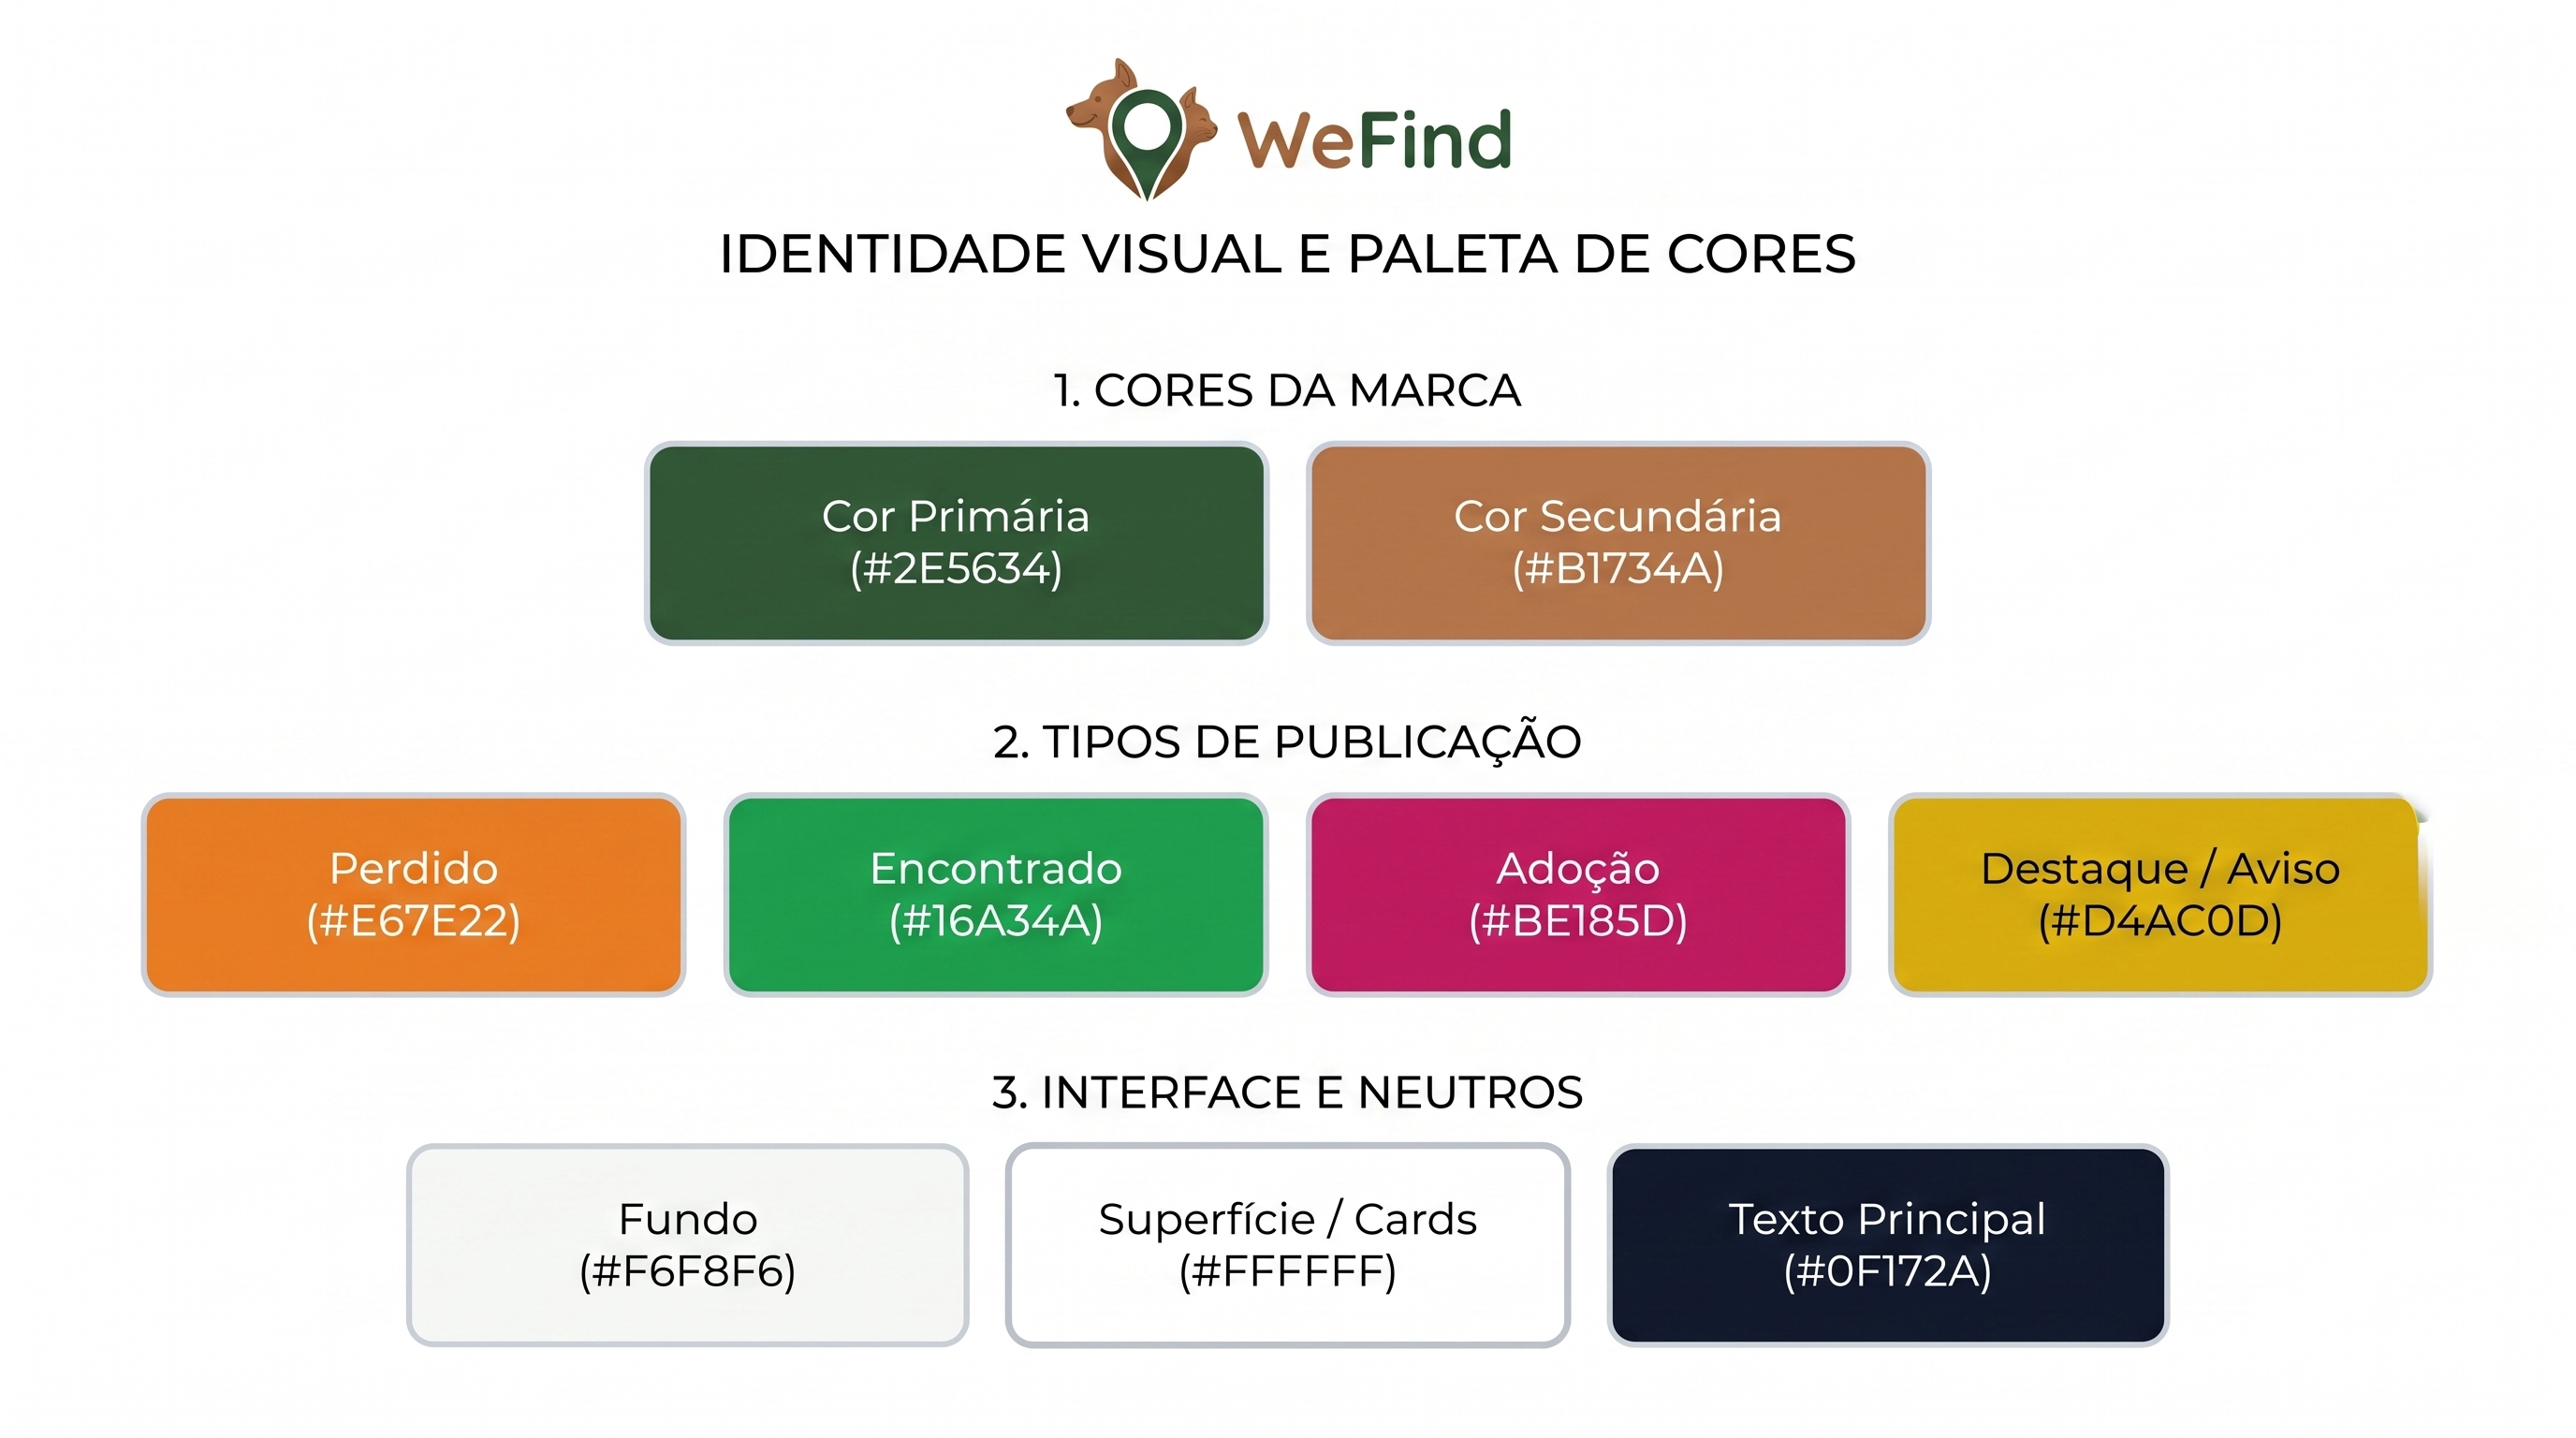
\includegraphics[width=0.88\textwidth]{imagens/03_arquitetura_design/figura14_paleta_cores.jpeg}
    \caption{Paleta Cromática Oficial do Sistema WeFIND}
    \label{fig:paleta_cores}
    \fonte{Autoria própria (2026)}
\end{figure}

As cores principais são formadas pela Cor Primária em tom Verde (\#2E5634), que evoca equilíbrio, esperança e solidez, aplicada nas barras de navegação superiores e botões primários; e pela Cor Secundária em tom Terracota (\#B1734A), associada ao acolhimento e cuidado com a vida animal, empregada em botões secundários e detalhes de realce.

Para a identificação visual imediata dos status dos animais no mapa e no feed, definiram-se quatro cores funcionais de contraste: Laranja Alerta (\#E67E22) para sinalizar animais com status Perdido, Verde Sucesso (\#16A34A) para animais Encontrados, Magenta (\#BE185D) para animais disponíveis para Adoção, e Amarelo Dourado (\#D4AC0D) para Avisos de novos avistamentos e publicações em destaque.

Por fim, os elementos neutros e de fundo adotam tonalidade cinza suave (\#F6F8F6) para evitar ofuscamento visual, áreas de superfície e cartões em branco puro (\#FFFFFF) para destacar fotografias e textos, e tipografia principal em tom azul escuro profundo (\#0F172A), garantindo contraste rigoroso em conformidade com o nível AA das diretrizes WCAG.

\subsection{Funcionamento e Telas do Aplicativo}

O WeFIND organiza suas funcionalidades em fluxos de interação diretos, orientados pela jornada prática do usuário e apoiados em uma barra de navegação inferior por abas. A Figura~\ref{fig:telas_autenticacao} ilustra o acesso inicial ao aplicativo, exibindo à esquerda a tela de autenticação (login por e-mail e senha com opção de redefinição de acesso) e à direita a tela de apresentação institucional (seção ``Conhecer a Plataforma''), que permite a exploração livre das ferramentas, visualização de depoimentos de reencontro e consulta a animais ativos antes do cadastro formal.

\begin{figure}[H]
    \centering
    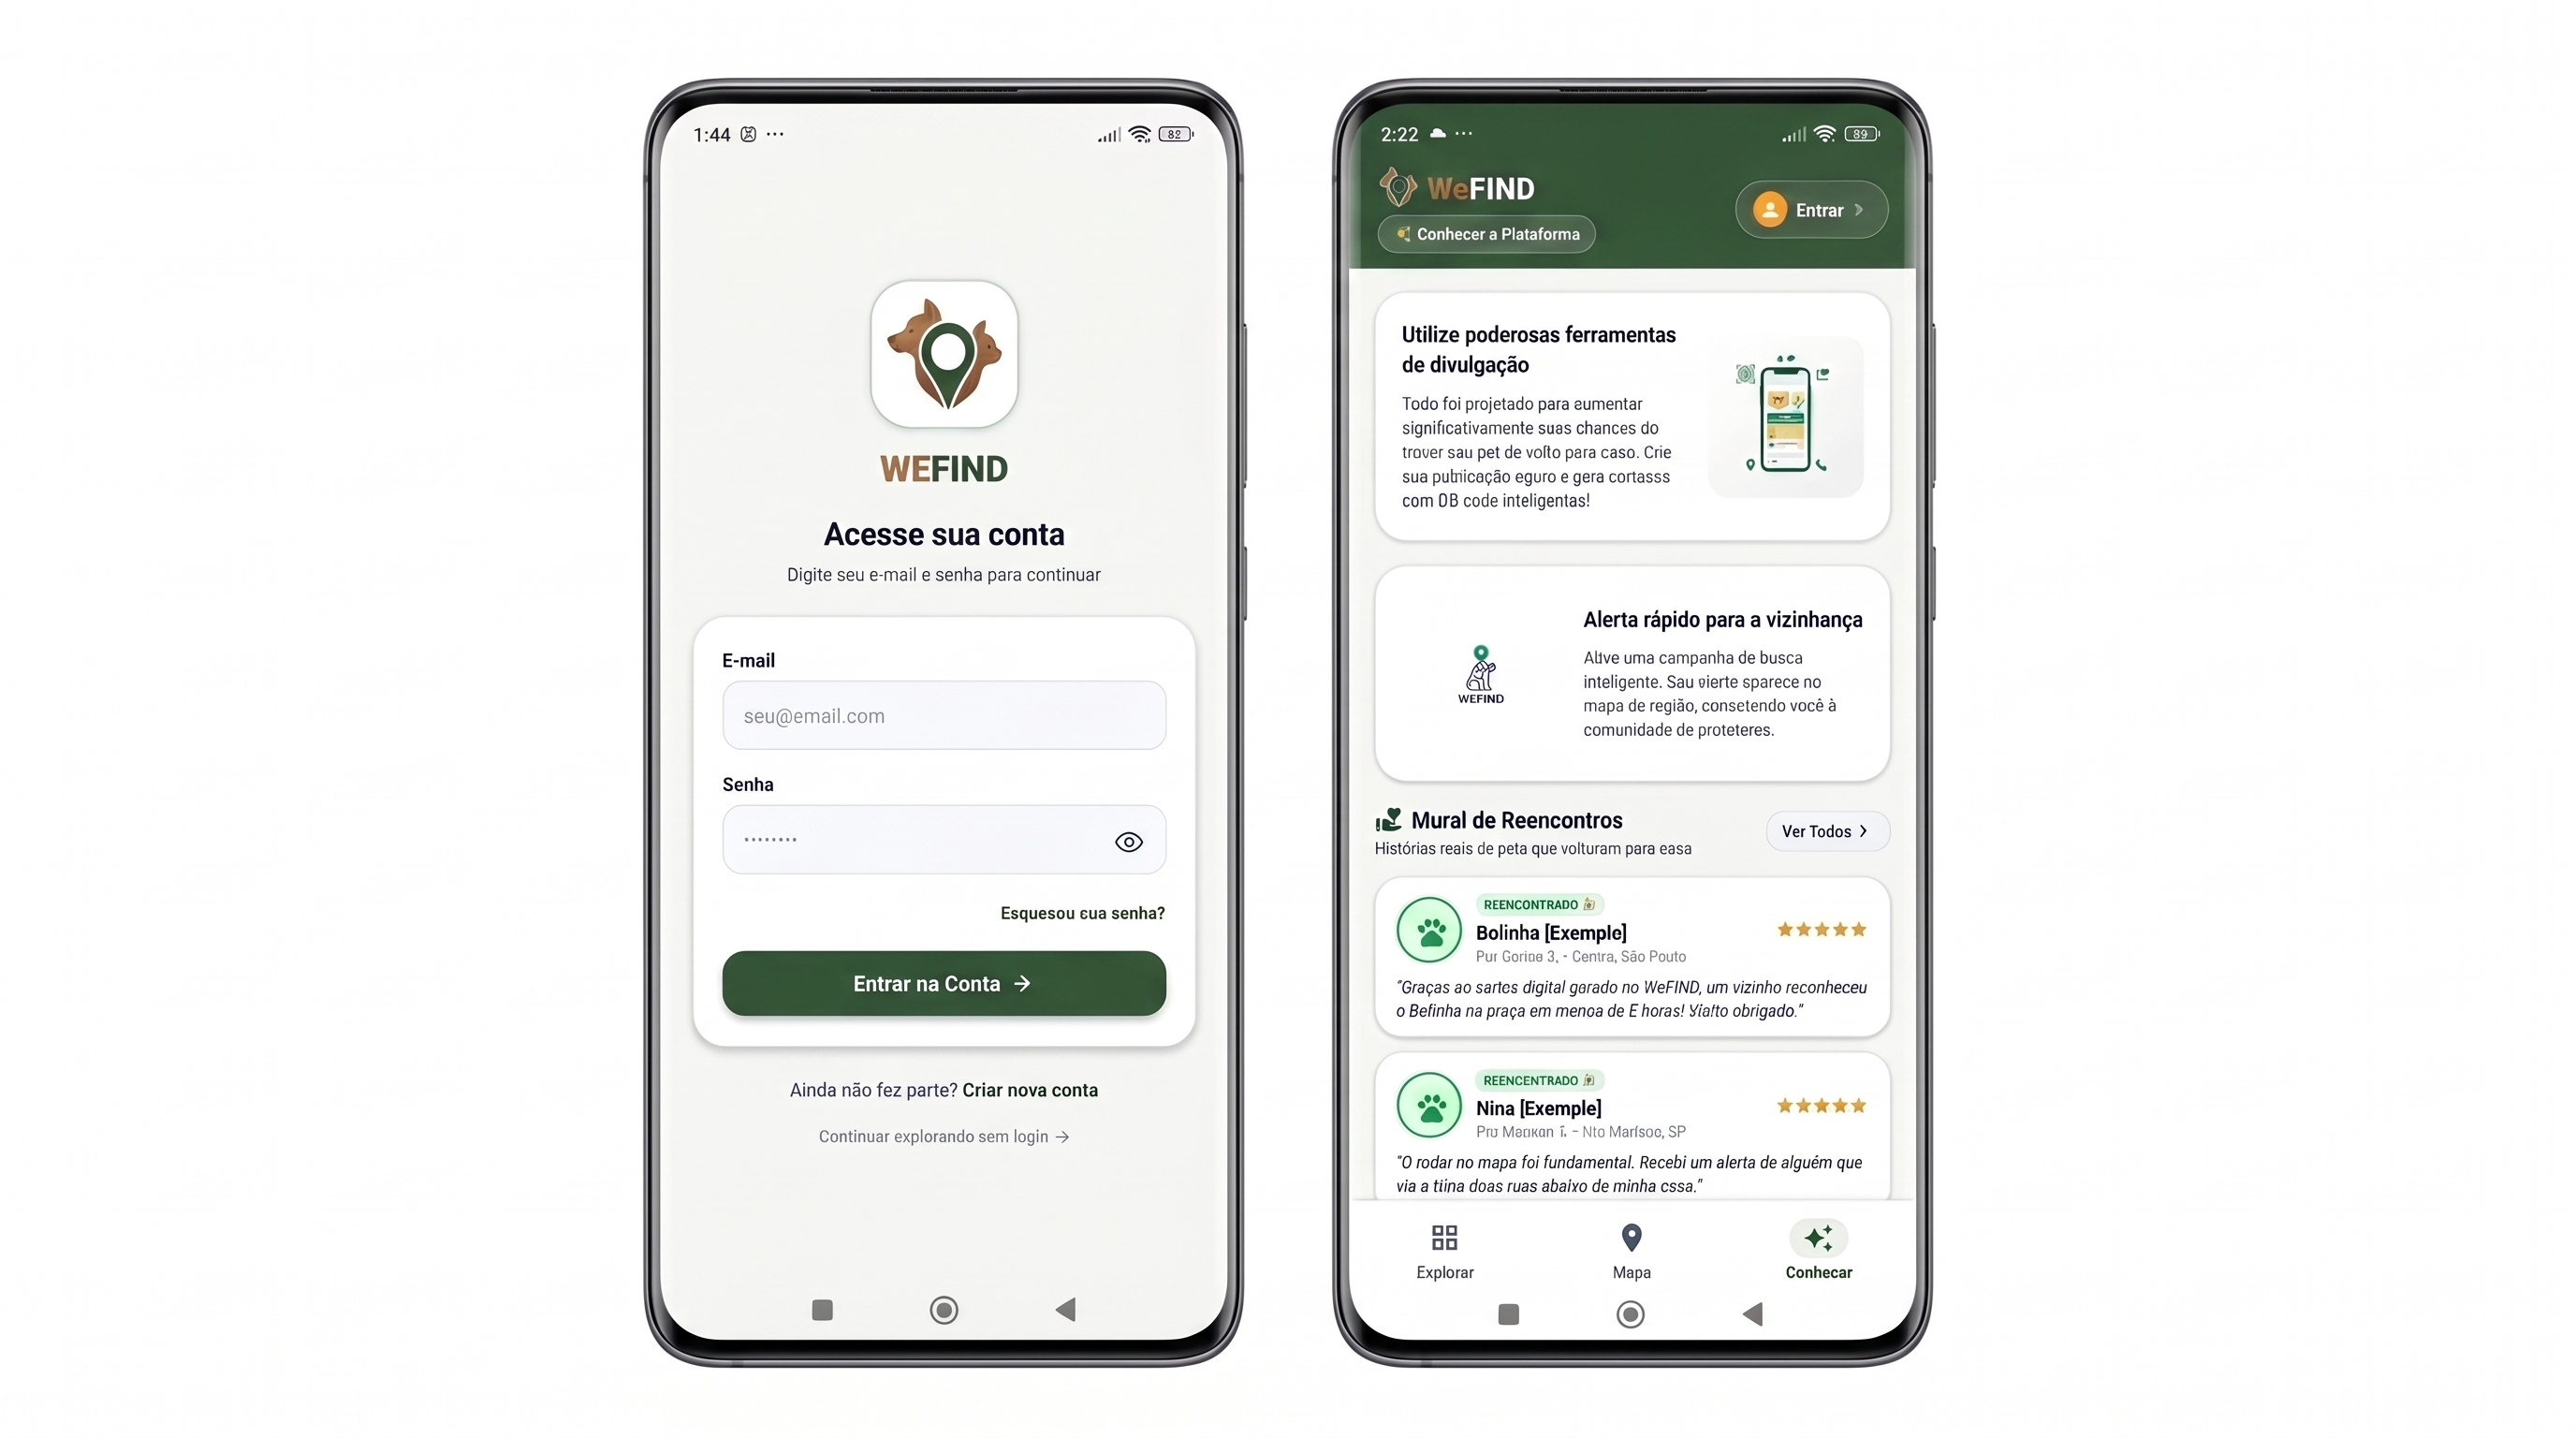
\includegraphics[width=0.99\textwidth]{imagens/04_telas_aplicativo/figura16_telas_autenticacao.jpeg}
    \caption{Telas de Autenticação (Login) e de Apresentação da Plataforma (Modo Conhecer)}
    \label{fig:telas_autenticacao}
    \fonte{Autoria própria (2026)}
\end{figure}

Após o ingresso na aplicação, o usuário é conduzido à tela inicial, apresentada na Figura~\ref{fig:tela_feed}. O feed reúne os anúncios recentes organizados em cartões informativos contendo fotografia em destaque, nome do pet, espécie, raça, tempo decorrido desde a publicação e distância aproximada em quilômetros até a posição atual do aparelho.

\begin{figure}[H]
    \centering
    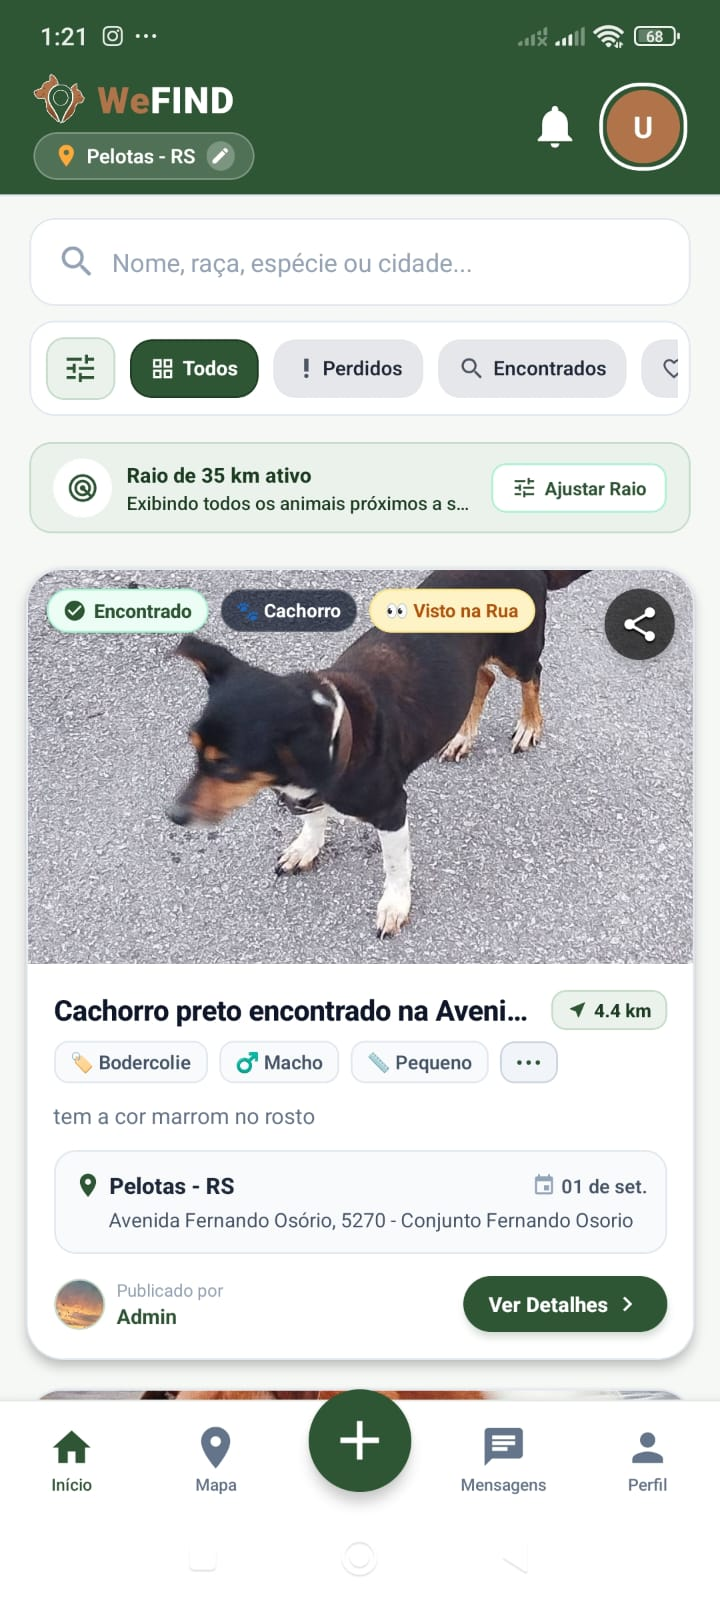
\includegraphics[width=0.45\textwidth]{imagens/04_telas_aplicativo/figura17_tela_feed.jpeg}
    \caption{Tela Inicial e Feed de Publicações de Animais Ativos}
    \label{fig:tela_feed}
    \fonte{Autoria própria (2026)}
\end{figure}

A navegação espacial em mapa interativo representa uma das principais funcionalidades do WeFIND. Como ilustrado na Figura~\ref{fig:tela_mapa}, o mapa exibe marcadores coloridos conforme a situação do animal, oferece ajuste de raio geográfico de busca e permite requisitar o cálculo de rotas viárias dinâmicas via GPS até o ponto onde o pet foi visto.

\begin{figure}[H]
    \centering
    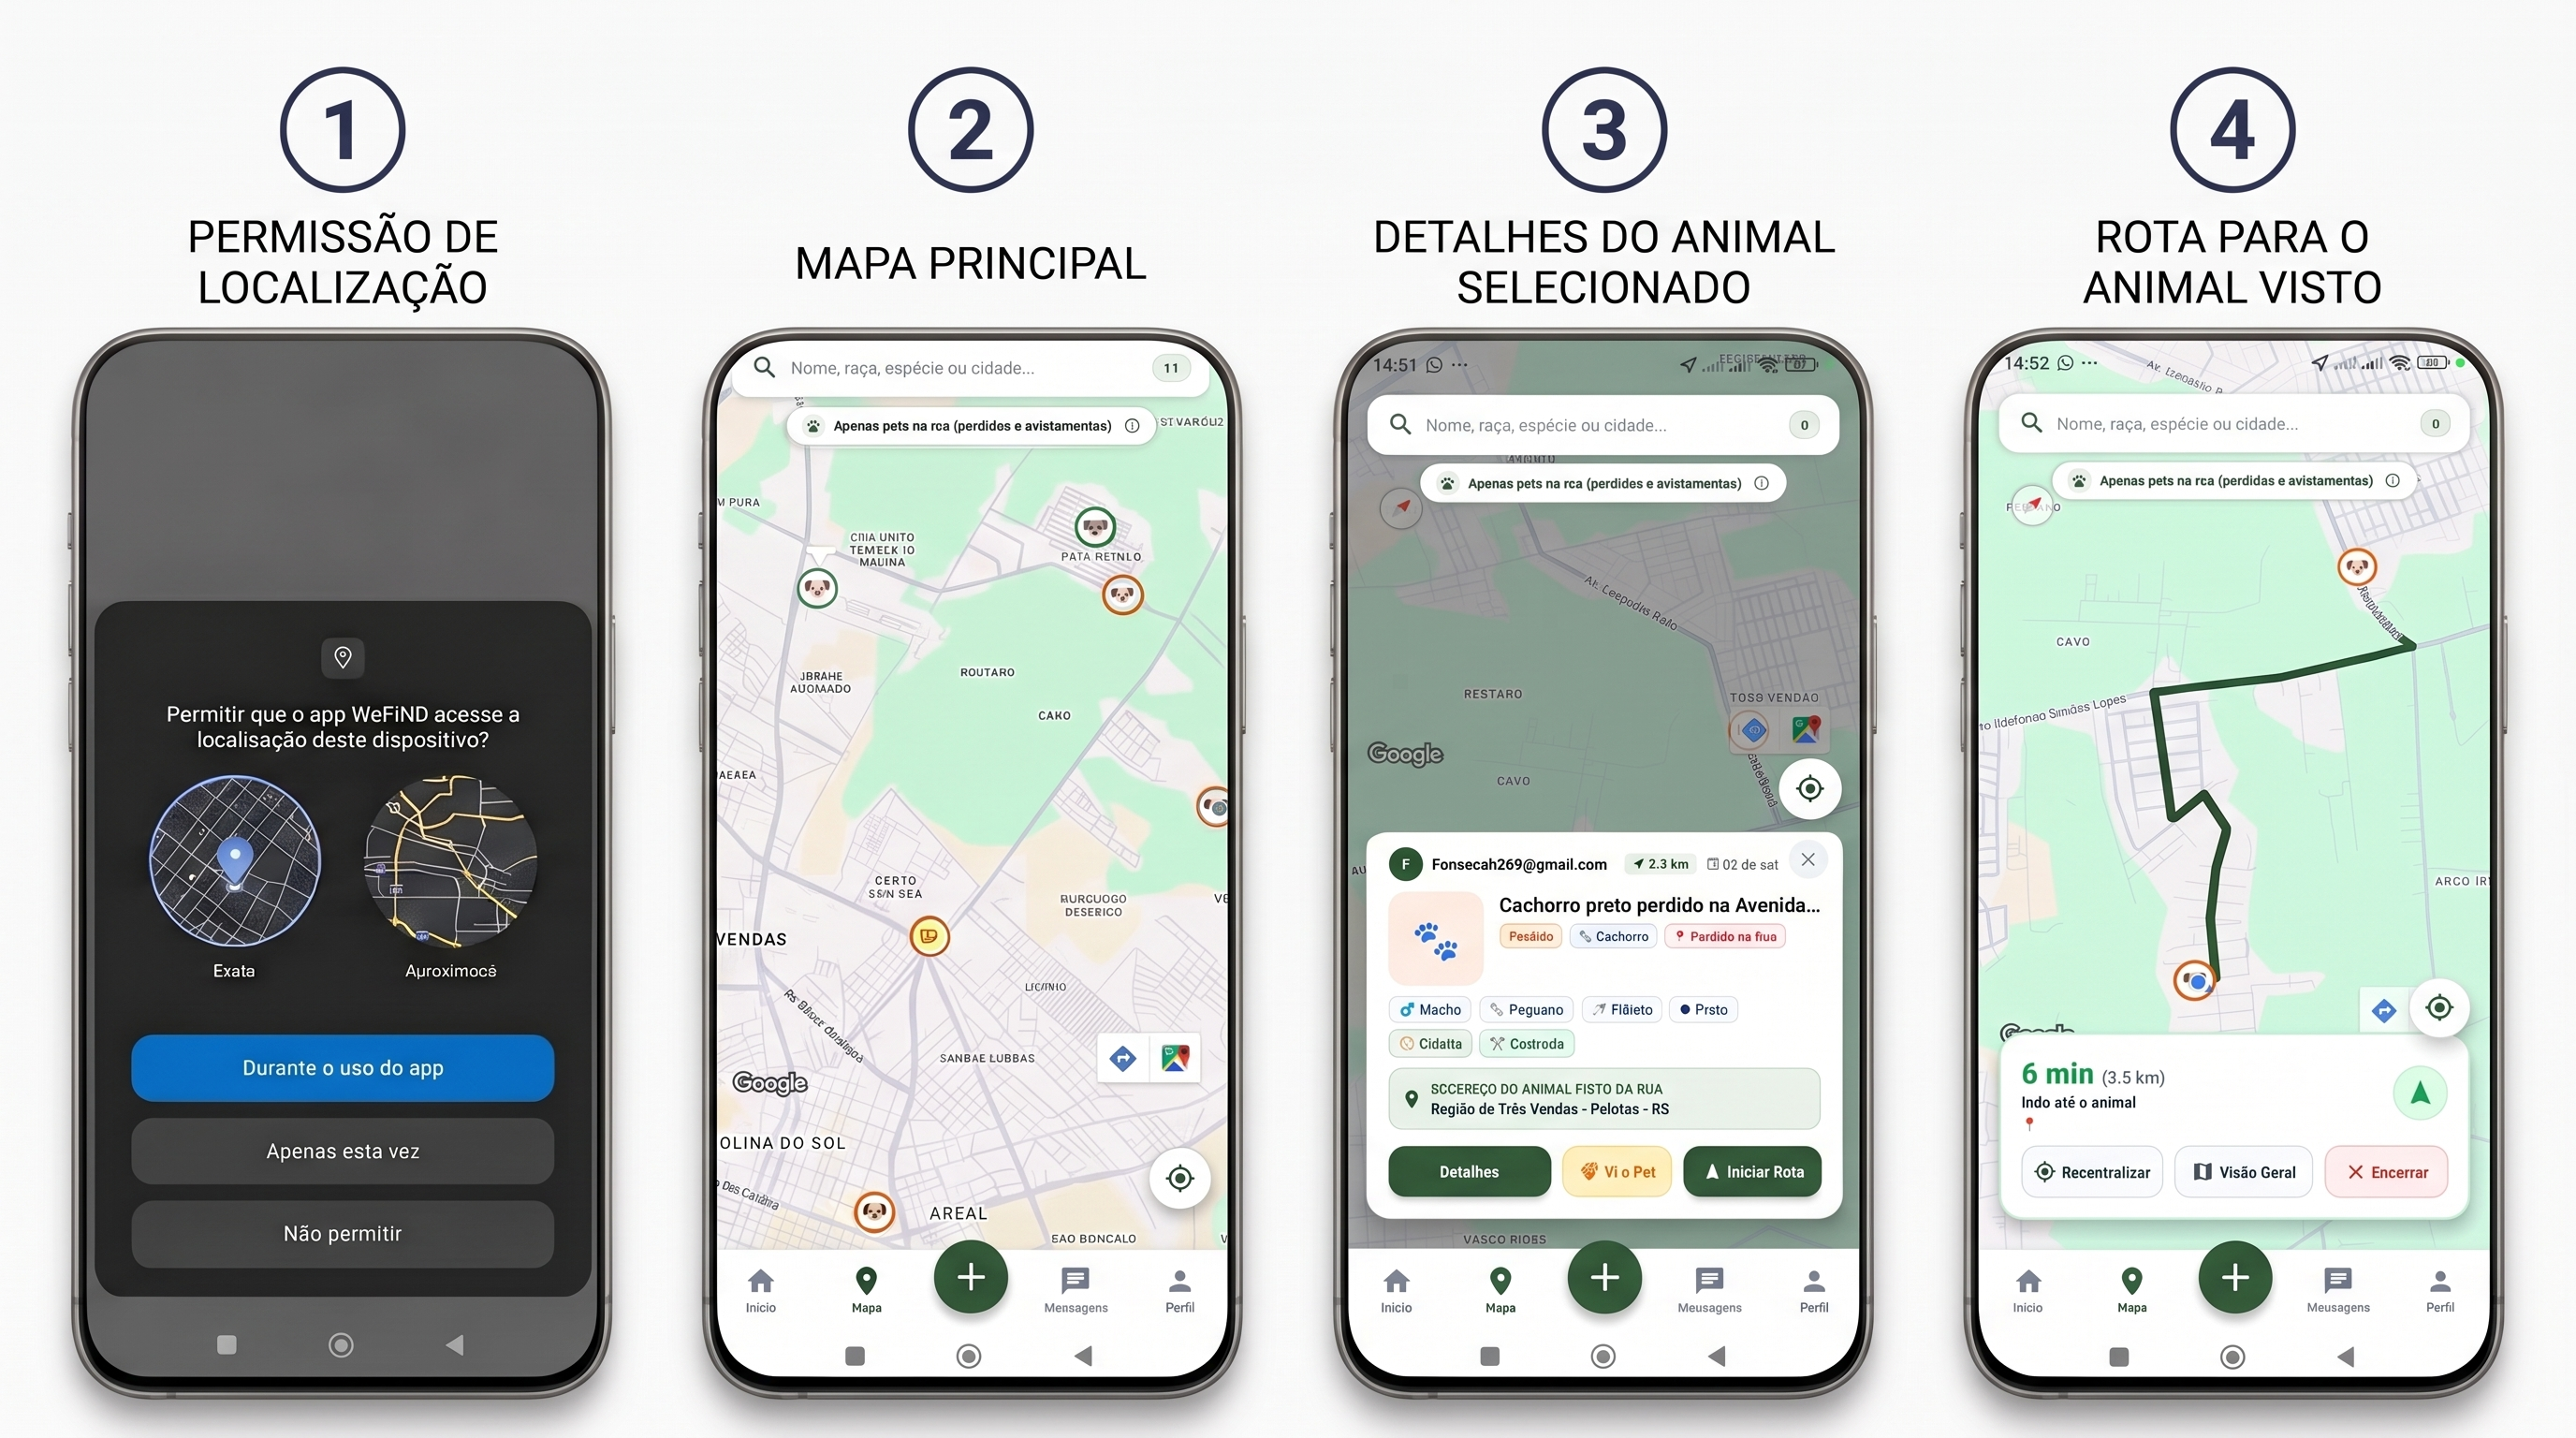
\includegraphics[width=0.98\textwidth]{imagens/04_telas_aplicativo/figura18_tela_mapa.jpeg}
    \caption{Fluxo de Utilização do Mapa Interativo e Traçado de Rotas GPS}
    \label{fig:tela_mapa}
    \fonte{Autoria própria (2026)}
\end{figure}

Ao tocar em qualquer cartão do feed ou marcador do mapa, abre-se a tela de detalhes completos da ocorrência (Figura~\ref{fig:tela_detalhes}). A tela concentra carrossel de fotos ampliadas, características físicas completas, histórico cronológico, botão para registro comunitário de avistamento e acesso ao bate-papo privativo com o anunciante.

\begin{figure}[H]
    \centering
    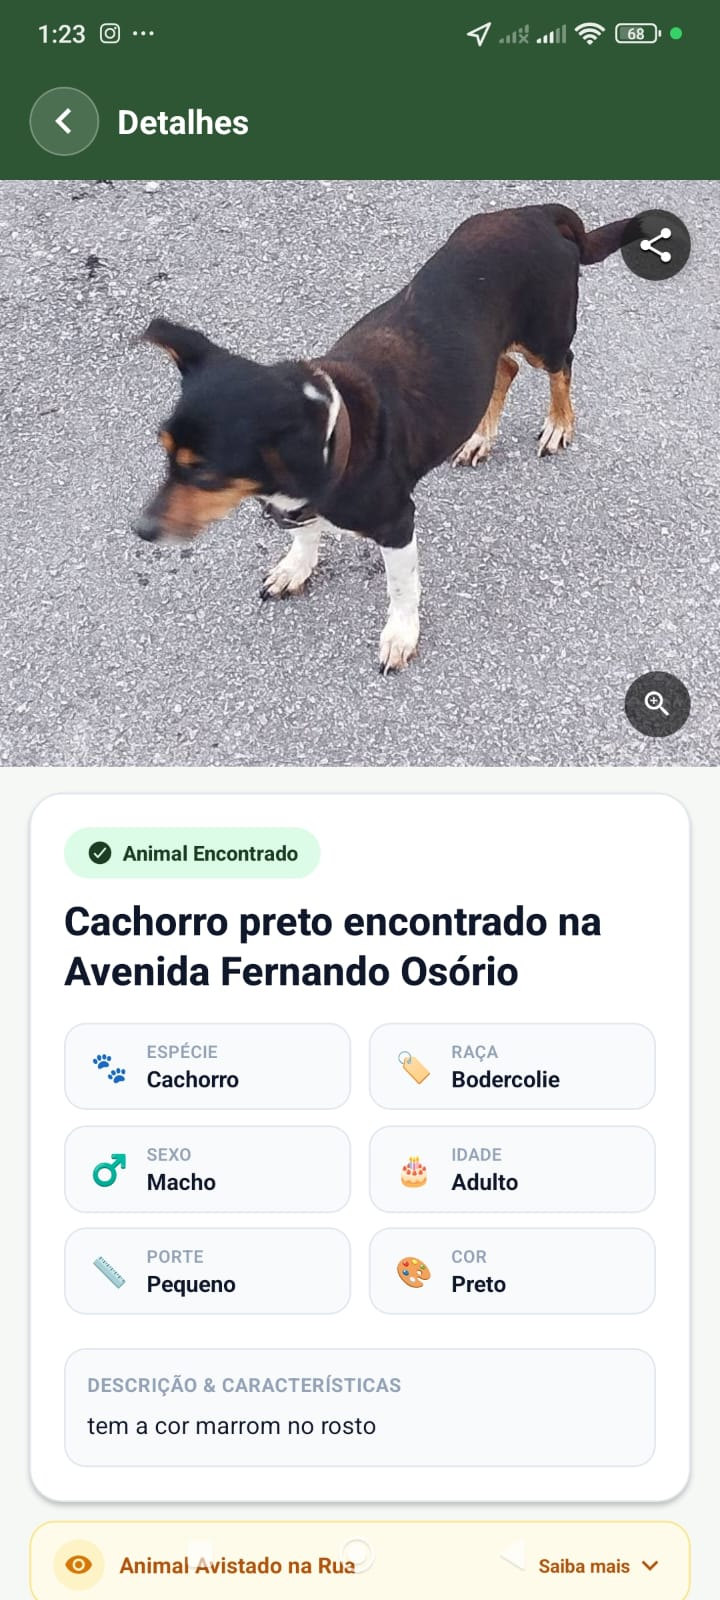
\includegraphics[width=0.45\textwidth]{imagens/04_telas_aplicativo/figura19_tela_detalhes.jpeg}
    \caption{Tela de Detalhes Completos da Publicação}
    \label{fig:tela_detalhes}
    \fonte{Autoria própria (2026)}
\end{figure}

Para registrar um novo anúncio, o aplicativo fornece o formulário ilustrado na Figura~\ref{fig:tela_cadastro}. O fluxo requer a indicação da categoria do fato (Perdido, Encontrado ou Adoção), anexo de fotografias capturadas na câmera ou obtidas na galeria, preenchimento das características individuais do animal e marcação direta do ponto geográfico em mapa interativo.

\begin{figure}[H]
    \centering
    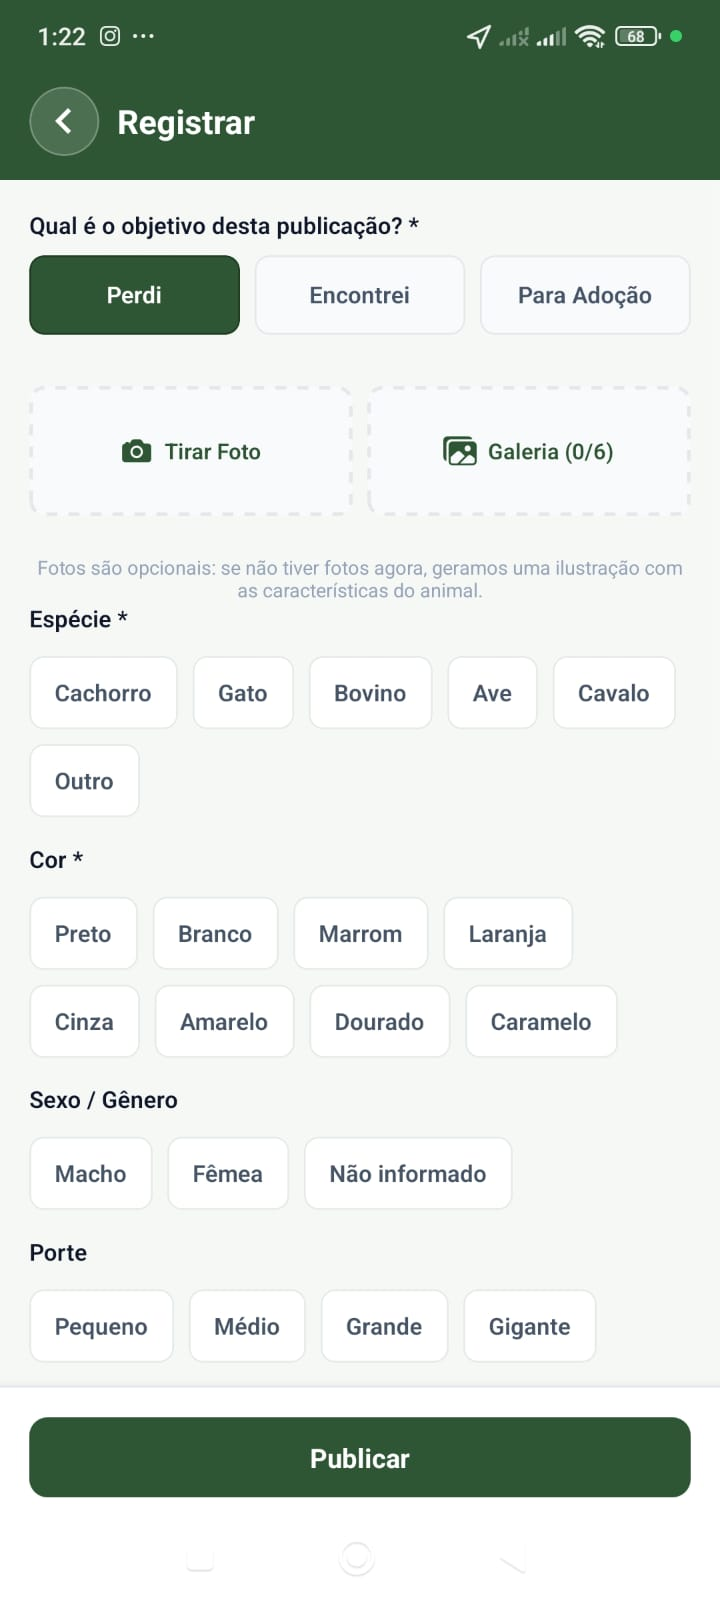
\includegraphics[width=0.45\textwidth]{imagens/04_telas_aplicativo/figura20_tela_cadastro.jpeg}
    \caption{Tela de Cadastro e Edição de Publicação de Animal}
    \label{fig:tela_cadastro}
    \fonte{Autoria própria (2026)}
\end{figure}

Como suporte às ações de divulgação externa, o sistema disponibiliza a geração automatizada de cartazes digitais de busca providos de código QR, conforme ilustrado na Figura~\ref{fig:tela_cartaz}. O recurso permite gerar o cartaz em formatos padronizados para impressão física ou para compartilhamento direto em aplicativos de redes sociais.

\begin{figure}[H]
    \centering
    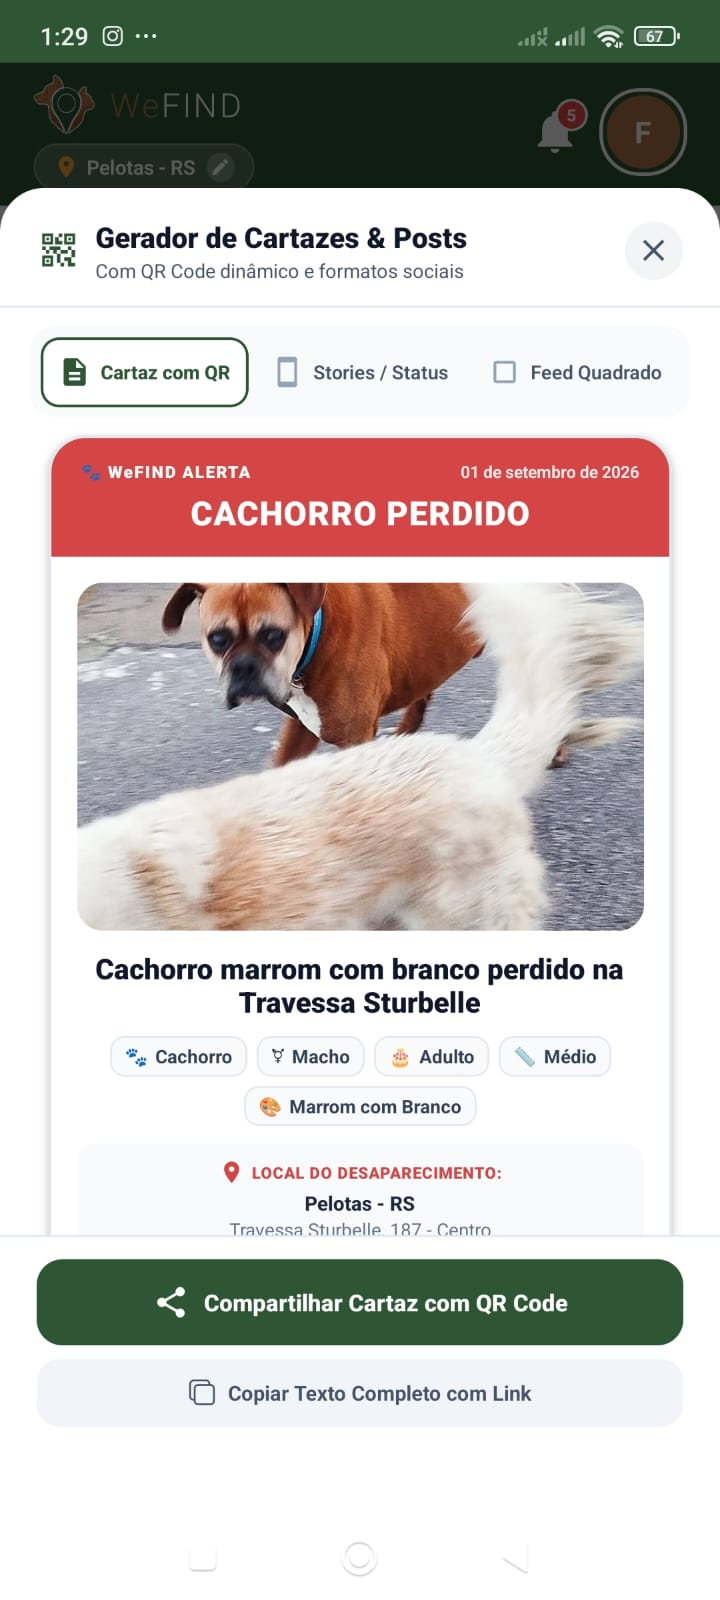
\includegraphics[width=0.45\textwidth]{imagens/04_telas_aplicativo/figura21_tela_cartaz.jpeg}
    \caption{Cartaz Digital de Busca de Animais com Código QR}
    \label{fig:tela_cartaz}
    \fonte{Autoria própria (2026)}
\end{figure}

Para intermediar o contato de forma segura entre a pessoa que encontrou o animal e o tutor que o procura, a aplicação integra o canal de bate-papo privativo em tempo real, apresentado na Figura~\ref{fig:tela_chat}. O chat resguarda a privacidade dos participantes ao eliminar a necessidade de exposição de números particulares de telefone.

\begin{figure}[H]
    \centering
    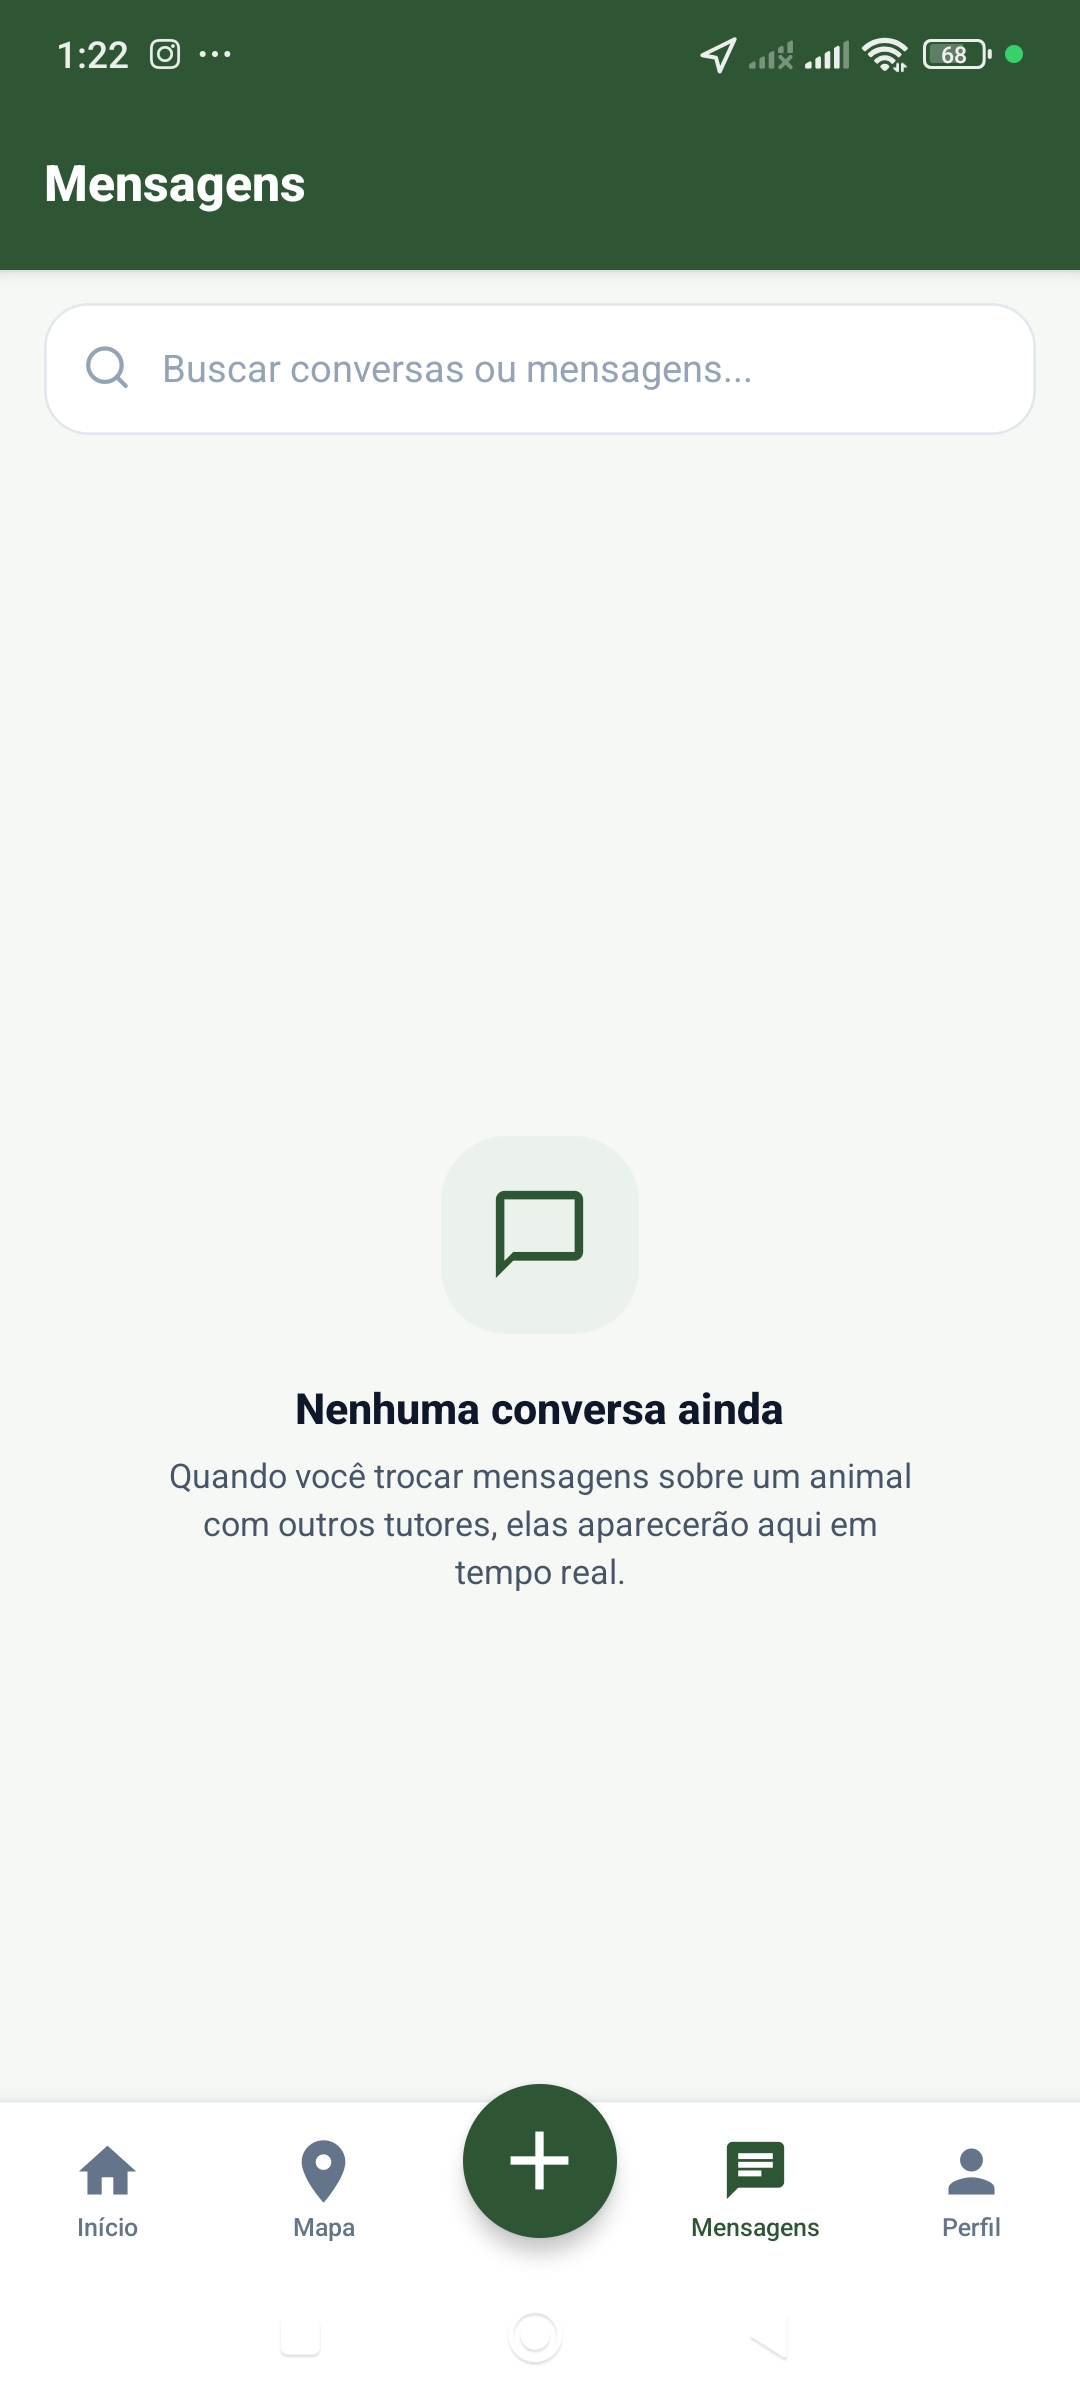
\includegraphics[width=0.45\textwidth]{imagens/04_telas_aplicativo/figura22_tela_chat.jpeg}
    \caption{Tela de Chat Privativo em Tempo Real}
    \label{fig:tela_chat}
    \fonte{Autoria própria (2026)}
\end{figure}

O refinamento das listagens tanto no feed quanto no mapa conta com o painel de filtros avançados apresentado na Figura~\ref{fig:tela_filtros}, viabilizando a seleção por espécie de animal, status do registro e raio de distância territorial.

\begin{figure}[H]
    \centering
    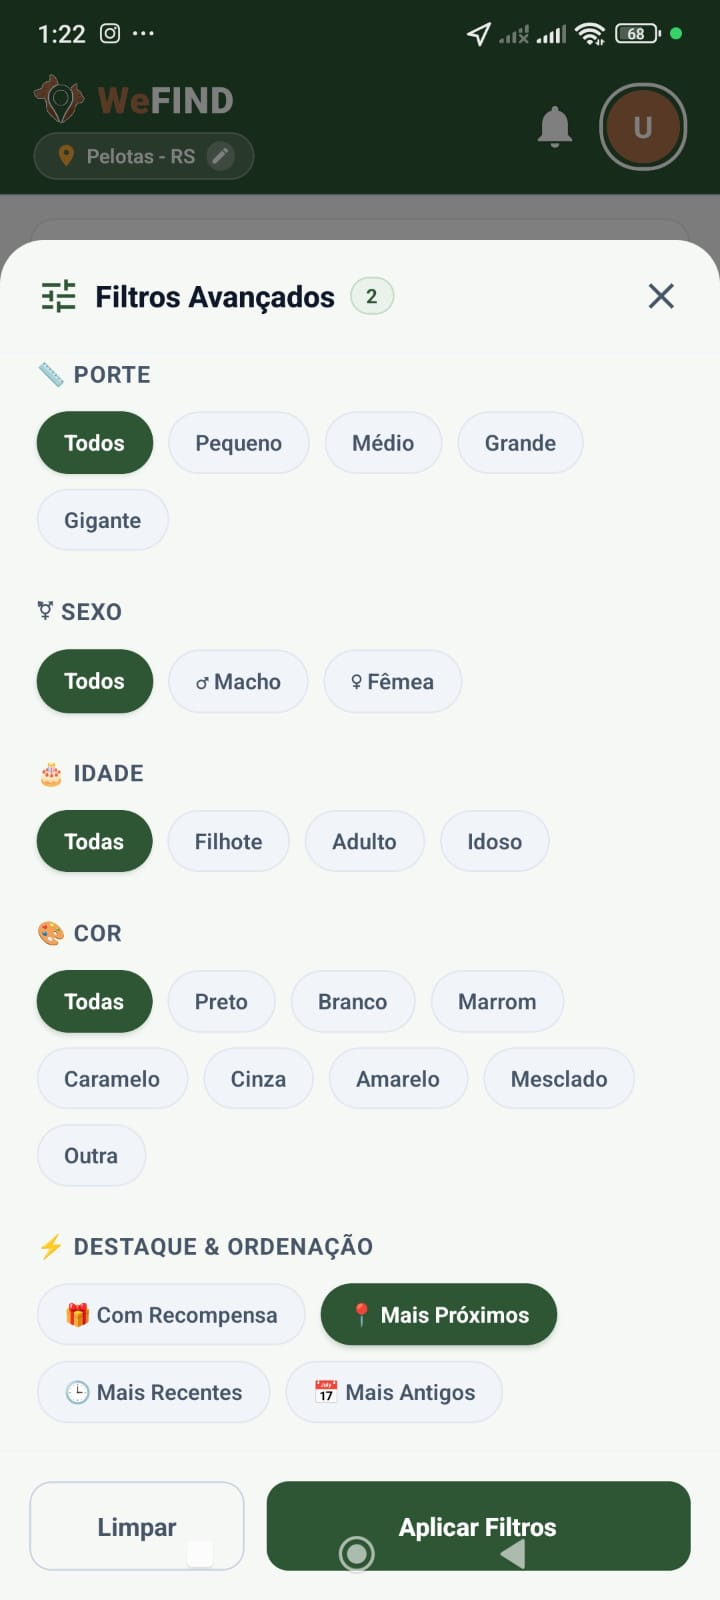
\includegraphics[width=0.45\textwidth]{imagens/04_telas_aplicativo/figura23_tela_filtros.jpeg}
    \caption{Painel de Filtros Avançados de Busca}
    \label{fig:tela_filtros}
    \fonte{Autoria própria (2026)}
\end{figure}

A tela de perfil do usuário (Figura~\ref{fig:tela_perfil}) centraliza a edição de dados cadastrais, o gerenciamento de publicações ativas e as conquistas de guardião, incentivando a colaboração contínua da comunidade.

\begin{figure}[H]
    \centering
    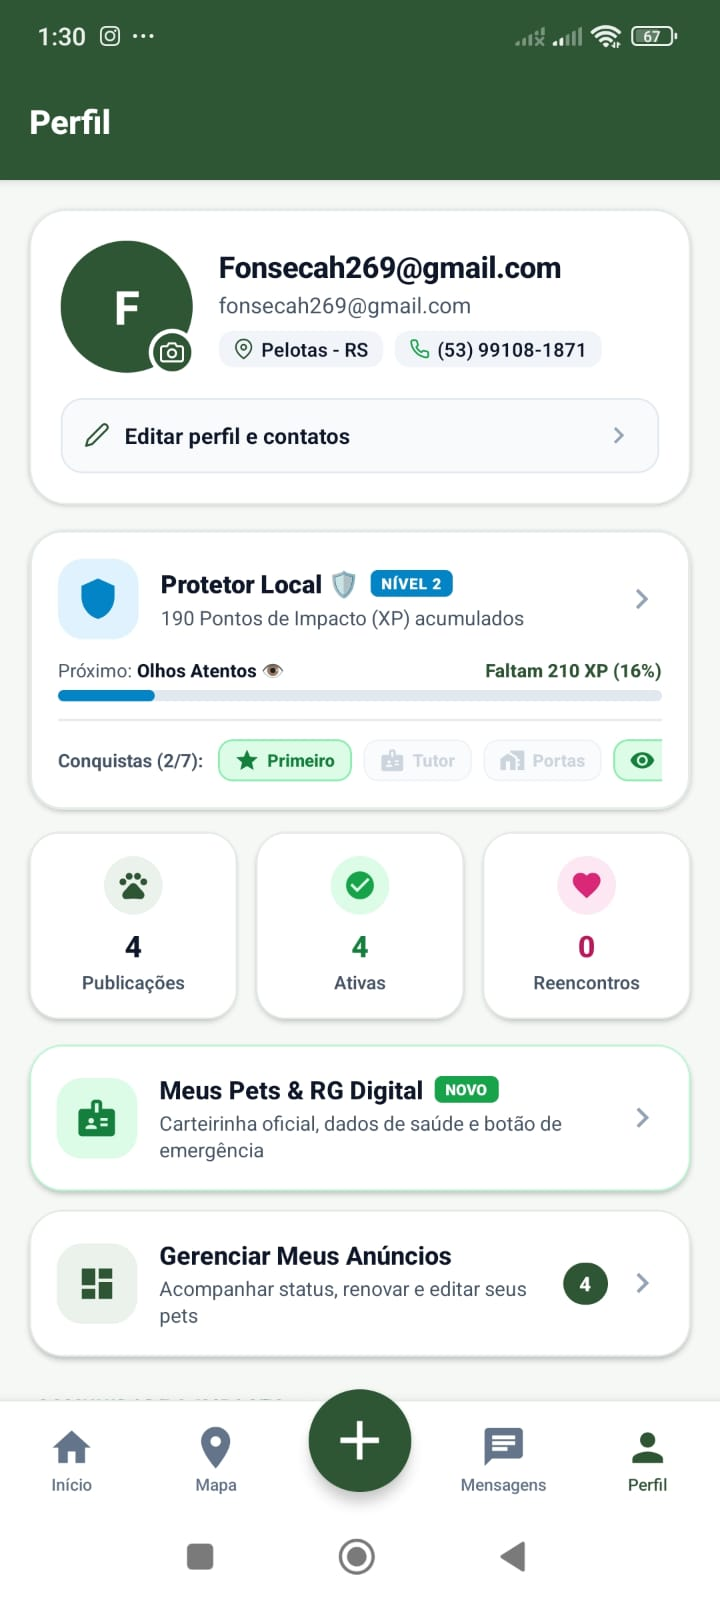
\includegraphics[width=0.45\textwidth]{imagens/04_telas_aplicativo/figura24_tela_perfil.jpeg}
    \caption{Tela de Perfil do Usuário e Conquistas de Guardião}
    \label{fig:tela_perfil}
    \fonte{Autoria própria (2026)}
\end{figure}

Por fim, a aplicação incentiva a guarda preventiva mediante o Perfil Digital do Pet, apresentado na Figura~\ref{fig:tela_perfil_pet}. Nessa interface, o tutor cadastra preventivamente seus animais domésticos, registrando histórico vacinal, fotos e gerando um código QR exclusivo para identificação rápida do animal.

\begin{figure}[H]
    \centering
    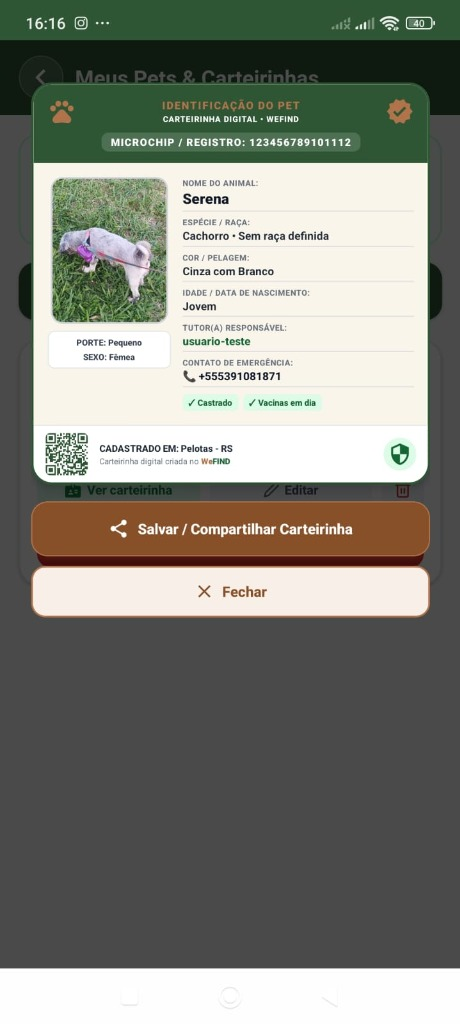
\includegraphics[width=0.45\textwidth]{imagens/04_telas_aplicativo/figura25_tela_rg_pet.jpeg}
    \caption{Tela do Perfil Digital do Pet}
    \label{fig:tela_perfil_pet}
    \fonte{Autoria própria (2026)}
\end{figure}

A consolidação de todas essas telas e componentes compõe a versão final executável do WeFIND. O Capítulo 7 apresenta o planejamento, a execução e os resultados dos testes funcionais e da avaliação de usabilidade realizados sobre a aplicação.
\clearpage
